% Editable TikZ diagram and equations transcribed from the lecture slide.
\subsection*{Double Pendulum on Cart: Model}

\begin{center}
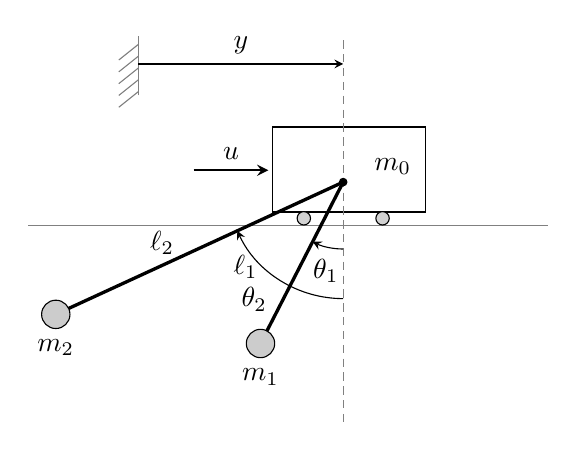
\begin{tikzpicture}[x=1cm,y=1cm,>=stealth]
  % Horizontal track and cart.
  \draw[gray] (-4,-0.55) -- (2.6,-0.55);
  \draw[fill=white] (-0.9,-0.38) rectangle (1.05,0.7);
  \node at (0.63,0.2) {$m_0$};
  \draw[fill=gray!35] (-0.5,-0.46) circle (0.085);
  \draw[fill=gray!35] (0.5,-0.46) circle (0.085);
  % Position reference and applied force.
  \draw[gray] (-2.6,1.1) -- (-2.6,1.85);
  \foreach \h in {1.15,1.3,1.45,1.6,1.75}
    \draw[gray] (-2.85,\h-0.2) -- (-2.6,\h);
  \draw[gray,densely dashed] (0,1.8) -- (0,-3.05);
  \draw[->] (-2.6,1.5) -- node[above] {$y$} (0,1.5);
  \draw[->,thick] (-1.9,0.15) -- node[above] {$u$} (-0.95,0.15);
  % Two independent pendulums share the pivot on the cart.
  \draw[very thick] (0,0) -- (-1.05,-2.05);
  \node at (-1.24,-1.08) {$\ell_1$};
  \draw[very thick] (0,0) -- (-3.65,-1.68)
    node[pos=0.63,above] {$\ell_2$};
  \fill (0,0) circle (0.055);
  \draw[fill=gray!40] (-1.05,-2.05) circle (0.18);
  \node[below] at (-1.05,-2.25) {$m_1$};
  \draw[fill=gray!40] (-3.65,-1.68) circle (0.18);
  \node[below] at (-3.65,-1.88) {$m_2$};
  % Angles are measured from the downward vertical towards the left.
  \draw[->] (0,-0.85) arc[start angle=-90,end angle=-117.12,radius=0.85];
  \node at (-0.22,-1.13) {$\theta_1$};
  \draw[->] (0,-1.48) arc[start angle=-90,end angle=-155.28,radius=1.48];
  \node at (-1.13,-1.49) {$\theta_2$};
\end{tikzpicture}
\end{center}

\noindent The equations of motion are
\[
\boxed{
\begin{aligned}
 &(m_0+m_1+m_2)\ddot y
 -m_1\ell_1\cos\theta_1\,\ddot\theta_1
 -m_2\ell_2\cos\theta_2\,\ddot\theta_2\\
 &\qquad +m_1\ell_1\sin\theta_1\,\dot\theta_1^{\,2}
 +m_2\ell_2\sin\theta_2\,\dot\theta_2^{\,2}=u,\\[6pt]
 &-m_1\ell_1\cos\theta_1\,\ddot y
 +m_1\ell_1^2\ddot\theta_1
 +m_1\ell_1g\sin\theta_1=0,\\[6pt]
 &-m_2\ell_2\cos\theta_2\,\ddot y
 +m_2\ell_2^2\ddot\theta_2
 +m_2\ell_2g\sin\theta_2=0.
\end{aligned}
}
\]
